Figure \ref{fig:softwareArchitecture} shows a high-level overview of the
software architecture at first granularity with the benchmarking system being
based on a message bus  architecture. The figure further shows the core
architectural components of the system.
\begin{figure}[H]
  \begin{center}
  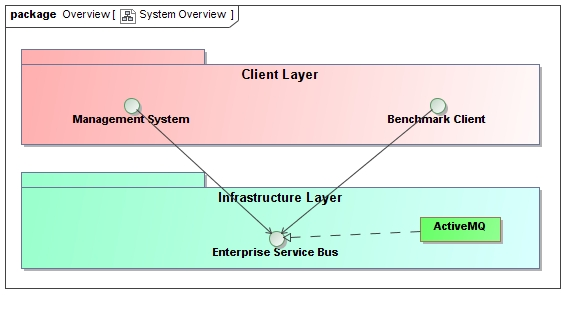
\includegraphics[scale=0.4]{../Diagrams and Charts/Overview/SystemOverview.jpg}
  \caption{A high-level overview of the software architecture for the Benchmarking Service at first granularity level}
  \label{fig:softwareArchitecture}
  \end{center}
\end{figure}

\section{Management System}
Figure \ref{fig:managementSoftwareArchitecture} shows a high-level overview of
the management service software architecture at second granularity level with the
service being based on a layered architecture. The figure further shows the core
architectural components of the subsystem.
\begin{figure}[H]
  \begin{center}
  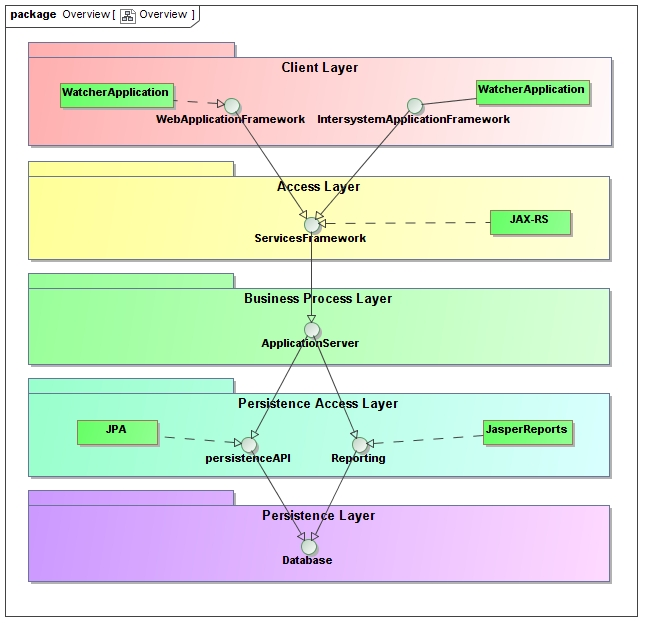
\includegraphics[scale=0.4]{../Diagrams and Charts/Overview/Overview.jpg}
  \caption{A high-level overview of the software architecture for the Management Service at second granularity}
  \label{fig:managementSoftwareArchitecture}
  \end{center}
\end{figure}

\section{Benchmark Client}
Figure \ref{fig:benchmarkSoftwareArchitecture} shows a high-level overview of
the benchmark service software architecture at second granularity level with the
service being based on a monolithic architecture. The figure further shows the core
architectural components of the subsystem.
\begin{figure}[H]
  \begin{center}
  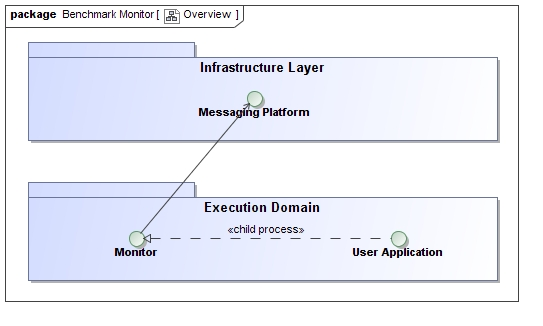
\includegraphics[scale=0.4]{../Diagrams and Charts/Overview/BenchmarkInfrastructure.jpg}
  \caption{A high-level overview of the software architecture for the Management Service at second granularity}
  \label{fig:benchmarkSoftwareArchitecture}
  \end{center}
\end{figure}
